\documentclass[a4paper,10pt]{article}
\usepackage[cm]{fullpage}

\usepackage[top=1cm, bottom=1cm, left=1cm, right=1cm]{geometry}%A Few Useful Packages
\usepackage{marvosym}
\usepackage{fontspec}					%for loading fonts
 
\usepackage{xunicode,xltxtra,url,parskip} 	%other packages for formatting
\RequirePackage{color,graphicx}
\usepackage[usenames,dvipsnames]{xcolor}
\usepackage{fullpage} 				%better formatting of the A4 page
% an alternative to Layaureo can be ** \usepackage{fullpage} **
\usepackage{supertabular} 				%for Grades
\usepackage{titlesec}					%custom \section
\usepackage{multirow}

\usepackage{array}
%Setup hyperref package, and colours for links
\usepackage{hyperref}


\marginparsep = 0pt
\marginparwidth = 2pt

\definecolor{linkcolour}{rgb}{0.9,0.2,0.6}

\hypersetup{pdfauthor=Sylvain Blot,
			pdfsubject=Resume,
			colorlinks,breaklinks,urlcolor=linkcolour,
			linkcolor=linkcolour}

%FONTS
\defaultfontfeatures{Mapping=tex-text}
\setmainfont[SmallCapsFont = Fontin SmallCaps]{Fontin}


%CV Sections inspired by: 
%http://stefano.italians.nl/archives/26
\titleformat{\section}{\Large\scshape\raggedright}{}{0em}{}[\titlerule]
\titlespacing{\section}{0pt}{3pt}{3pt}
%Tweak a bit the top margin
%\addtolength{\voffset}{-1.3cm}

%Italian hyphenation for the word: ''corporations''
\hyphenation{im-pre-se}

%-------------WATERMARK TEST [**not part of a CV**]---------------
%\usepackage[absolute]{textpos}

%\setlength{\TPHorizModule}{30mm}
%\setlength{\TPVertModule}{\TPHorizModule}
%\textblockorigin{2mm}{0.65\paperheight}
%\setlength{\parindent}{0pt}

%--------------------BEGIN DOCUMENT----------------------
\begin{document}

\pagestyle{empty} % non-numbered pages

%--------------------TITLE-------------
%\begin{tabular}[t]{p{7cm}p{10cm}}
%\Huge \textsc{Sylvain Blot} \\ \huge \textsc{Ingénieur Système} &  \normalsize \textsc{146 boulevard du Montarpasse - 75014 Paris} \\ \Large{\Letter}\large{\href{mailto:sylvain.blot@gmail.com}{sylvain.blot@gmail.com}} \\ \Large{\Telefon} \large{+ 33 6 75 86 87 19}\\ \normalsize \textsc{12 Février 1985 - Permis B} \\
%\end{tabular}


\begin{tabular}[T]{p{4cm}p{8,2cm}p{3cm}}
 \LARGE{\textsc{Sylvain Blot}}\newline \Large{\textsc{System Engineer}} & \normalsize{\textsc{6 rue du Jeu de Paume - 67000 Strasbourg}} \newline \Large{\Letter} \large{\href{mailto:sylvainblot@me.com}{sylvainblot@me.com}} \Large{\Telefon} \large{+ 33 6 75 86 87 19} \newline \normalsize{\textsc{12 Février 1985 - Driving Licence}}
\newline \normalsize{\textsc{French, English, German (basic)}} &\parbox[c]{1em}{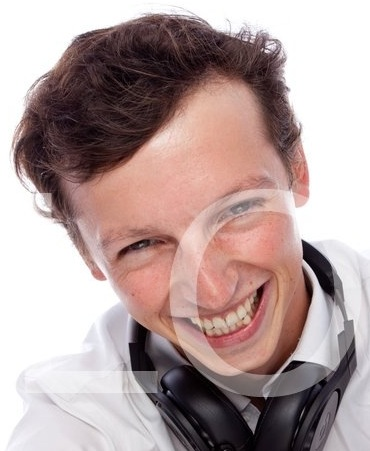
\includegraphics[width=0.20\textwidth,angle=5]{sylvain.jpg} }
\end{tabular}
\par Computer by choice
%--------------------SECTIONS-----------------------------------
%Section: Work Experience at the top
\section{Experiences}
%\begin{tabular}{r|p{11cm}}
\begin{tabular}{p{3,5cm}|p{15,5cm}}	

%FreeLance
	\emph{September 2013} & \textsc{Web Project Manager, Smile Inductries}, Strasbourg \\\textsc{September 2012}&\emph{ERP, CRM, eCommerce Solution. Managing a Team of 5 people}\\&\footnotesize{Enhance security, versioning, continuous integration, deployement.}\\\multicolumn{2}{c}{} \\

%FreeLance
	\emph{September 2012} & \textsc{Freelance Web Project Management}, Strasbourg \\\textsc{July 2011}&\emph{Future Exchange graphics, hotel booking solution}\\&\footnotesize{Django, Drupal, Expression Engine.}\\\multicolumn{2}{c}{} \\

  \emph{June 2011} & Project Manager, \textsc{SdV Plurimédia}, Strasbourg \\\textsc{July 2012}&\emph{ In charge of the tourism division and CMS Research and development  }\\&\footnotesize{Architect and developer of a modern tourism solution to enrich and sell travels.}\\\multicolumn{2}{c}{} \\
  
%Mallyance
 \emph{September 2008} & System and Network Engineer, \textsc{Mallyance}, Paris \\\textsc{April 2010}&\emph{Technical Project Manager for France Télécom - GOA}\\&\footnotesize{Managing Warhammer Online game infrastructure.}\\\multicolumn{2}{c}{} \\
%Prestige
 \emph{December 2006} & First professional experience at \textsc{Prestige Réseaux}, Suresnes \\\textsc{September 2007}&\emph{Linux consultant and trainer}\\&\footnotesize{Training \emph{Novell} Linux partners, different kind of consulting missions for big companies.}\\\multicolumn{2}{c}{} \\
%Supinfo SCT
 \emph{Septembre 2005} & Certified \textsc{SUPINFO} Linux Trainer, Strasbourg \\\textsc{Juin 2007}&\emph{Linux et Sun Solaris technologies trainer.}\\&\footnotesize{Training \emph{ESI Supinfo} students (until Master degree).}\\\multicolumn{2}{c}{}
%\textsc{Summer 2007} & Summer Intern at \textsc{Lehman Brothers}, \emph{Capital Markets}\\&\footnotesize{Received pre-placed offer from the Exotics Trading Desk as a result of very positive review. Rated ``\emph{truly distinctive}'' for Analytical Skills and Teamwork.}
\end{tabular}

%Section: Scholarships and additional info
%\section{Scholarships and Certificates}
%\begin{tabular}{rl}
% \textsc{Sept.} 2006 & Scholarship for graduate students with an outstanding curriculum \footnotesize(\EURcr 30,000)\normalsize\\
%\textsc{June} 2006 & {\textsc{Gmat}\textregistered}\setmainfont[SmallCapsFont=Fontin SmallCaps]{Fontin-Regular}: 730 (\textsc{q:50;v:39}) 96\textsuperscript{th} percentile; \textsc{awa}: 6.0/6.0 (89\textsuperscript{th} percentile)
%\end{tabular}

%Section: Languages
\section{Skills and Interest}
\begin{tabular}{p{2,5cm}|p{12,5cm}}	
\textsc{OS} & Mac OS, Linux, Unix (Solaris, *BSD), Windows\\
\textsc{Languages} & C, Shell script (BaSH, Python, Perl), JAVA, HTML, PHP, Javascript, CSS, SQL,\LaTeX\\
\textsc{Services} & OpenSSH, DNS (BIND), LDAP, NFS, OpenSSL, SAMBA, IPTABLES, Kerberos, MySQL, Apache\ldots\\
\textsc{Interests} & Literature, Raspberry PI hack\ldots\\
\textsc{Sports} & running, tennis, football\ldots
\end{tabular}


%Section: Education
\section{Education}
%\begin{tabular}{rl}	
%\begin{tabular}{r|p{11cm}}
\begin{tabular}{p{3,5cm}|p{12,5cm}}	
\multirow{1}*{\parbox[c]{1em}{
\includegraphics[width=0.15\textwidth]{brookes.pdf}}} & Master of Science in \textsc{Computer Science}, \textbf{Oxford Brookes University}, Oxford\\
 &\normalsize \textbf{Graduated with Distinction}, Member of the British Computer Society\\
& Dissertation: ``Finger tracking Desktop Experience'' | \small Supervisor: Doctor Philip \textsc{Torr}\\
& Research to replace the mouse by tracking fingers on the air\\
\textsc{September} 2007& Fully Working project written in Python including Linux GUI and AI.\\
\textsc{September} 2008& Fields: Distributed Systems, AI, Compiler construction, Software production\\
&\\\multicolumn{2}{c}{} \\
 \textsc{September} 2003 & \textsc{Computer} Engineer, \textbf{ESI Supinfo}, Strasbourg\\
\textsc{September} 2008 & Expert in information systems \\
 \multirow{1}*{\parbox[c]{1em}{
\includegraphics[width=0.15\textwidth]{supinfo.pdf}}}

 & OS : Linux, Microsoft, Apple; Network; Databases Oracle; Development, Management \\\multicolumn{2}{c}{} 
\end{tabular}

%\newpage
%\hypertarget{gmat}{\textsc{Gmat}\setmainfont{LMRoman10 Regular}\textregistered\setmainfont[SmallCapsFont=Fontin-SmallCaps]{Fontin-Regular}}

%\XeTeXpdffile ''GMAT.pdf'' page 1 scaled 800

\end{document}
